\documentclass[14pt]{article}

\usepackage[utf8x]{inputenc}
\usepackage[russian]{babel}
\usepackage{graphicx}
\graphicspath{{images/}}
\DeclareGraphicsExtensions{.pdf,.png,.jpg,.jpeg}

\usepackage{amsmath}
\usepackage{multirow}
\usepackage{pgfplots}

\usepackage{geometry} % Меняем поля страницы
\geometry{left=2cm}% левое поле
\geometry{right=1.5cm}% правое поле
\geometry{top=2cm}% верхнее поле
\geometry{bottom=2cm}% нижнее поле

\renewcommand{\theenumi}{\arabic{enumi}}% Меняем везде перечисления на цифра.цифра
\renewcommand{\labelenumi}{\arabic{enumi}}% Меняем везде перечисления на цифра.цифра
\renewcommand{\theenumii}{.\arabic{enumii}}% Меняем везде перечисления на цифра.цифра
\renewcommand{\labelenumii}{\arabic{enumi}.\arabic{enumii}.}% Меняем везде перечисления на цифра.цифра
\renewcommand{\theenumiii}{.\arabic{enumiii}}% Меняем везде перечисления на цифра.цифра
\renewcommand{\labelenumiii}{\arabic{enumi}.\arabic{enumii}.\arabic{enumiii}.}% Меняем везде перечисления на цифра.цифра

\begin{document}
\begin{titlepage}
	\begin{center}
		\fontsize{18pt}{20pt}\selectfont
		\textbf{Работа 1.4.4.}	
	
		\vspace{5cm}
		\fontsize{24pt}{25pt}\selectfont
		Определение скорости полета пули при помощи баллистического маятника
	\end{center}
	\begin{flushright}
		\fontsize{18pt}{20pt}\selectfont
		\vspace{14cm}
		\hspace{-3cm}
		\textit{Корнеев Е.С.}
	\end{flushright}		
\end{titlepage}

\begin{center}
	\fontsize{16pt}{18pt}\selectfont	
	Определение скорости полета пули при помощи баллистического маятника
\end{center}

\fontsize{14pt}{16pt}\selectfont
\vspace{1cm}
\textbf{Цель работы:} определить скорость полета пули, применяя законы сохранения и используя баллистические матяники.

\vspace{0.5cm}
\textbf{В работе используются:} духовое ружье на штативе, осветитель, оптическая система для измерения отклонений маятника, измерительная линейка, пули и весы для их взвешивания, баллистические маятники.

\vspace{1cm}
Скорость вылета нули из духового ружья $150 - 200$ м/с, из боевой винтовки - $1000$ м/с.


Это скорости большие по сравнению, скажем, со скоростью пешехода ($\sim 2$ м/с) или даже автомобиля ($\sim 20$ м/с). Поскольку размер лабораторной установки обычно порядка нескольких метров, время пролета пули составляет величину порядка $10^{-2} - 10^{-3}$ с. Для измерения таких величин необходима. дорогостоящая аппаратура, регистрирующая быстропеременные процессы. Дешевле определить скорость пули по импульсу, передаваемому ею некоторому телу при неупругом соударении. В отсутствие внешних сил, а при кратковременном ударе даже и при действии внешних сил, импульс системы пуля-тело сохраняется. Если масса тела значительно больше массы пули, то скорость тела с застрявшей в нем пулей будет значительно меньше скорости пули, и ее легче измерить. Длительность неупругого соударения пули и тела, измеряемая с момента их соприкосновения, зависит от сопротивления, которое испытывает пуля при движении внутри тела. Оценить ее можно по глубине проникновения нули в тело, предполагая силу сопротивления постоянной. Если при скорости $200$ м/с глубина. проникновения $\sim 1$ см, то время соударения $\sim 10^{-4}$ с. За это время даже тело только в $100$ раз более тяжелое, чем пуля, сдвинется всею на $0.1$ мм. При малых временах соударения внешние силы конечной величины сообщают импульс, намного меньший импульса пули.

Для измерения переданного пулей импульса и, следовательно, ее скорости, используют баллистический маятник. Баллистическим называется маятник, колебания которого вызываются кратковременным начальным импульсом (толчком). Кратковременным можно считать импульс, если время действия сил (время соударения) значительно меньше периода колебаний маятника. При этом отклонение маятника за время соударения значительно меньше амплитуды колебаний - максимального отклонения маятника. В случае гармонических колебаний время соударения $\tau$, отнесенное к периоду колебаний $T$, и отклонение $\Delta\varphi$ за время соударения, отнесенпое к максимальному отклонению $\varphi_m$(амплитуде), связаны простым соотношением

$$
	\frac{\Delta\varphi}{\varphi_m} \approx \frac{2\pi\tau}{T}
$$

\noindent B результате если время соударения составляет $0.01$ периода, то отклонение равно $0,06$ максимального отклонения. 

Связь между максимальным отклонением маятника и начальной скоростью, полученной им в результате толчка, описывается законом сохранения механической энергии, если потери энергии за период значительно меньше энергии его колебаний. В дальнейшем будем считать затухание малыми, если за десять колебаний амплитуда уменьшается меньше, чем наполовину. По начальному максимальному отклонению маятника определяются импульс и скорость пули.

\begin{figure}[h!]
	\center{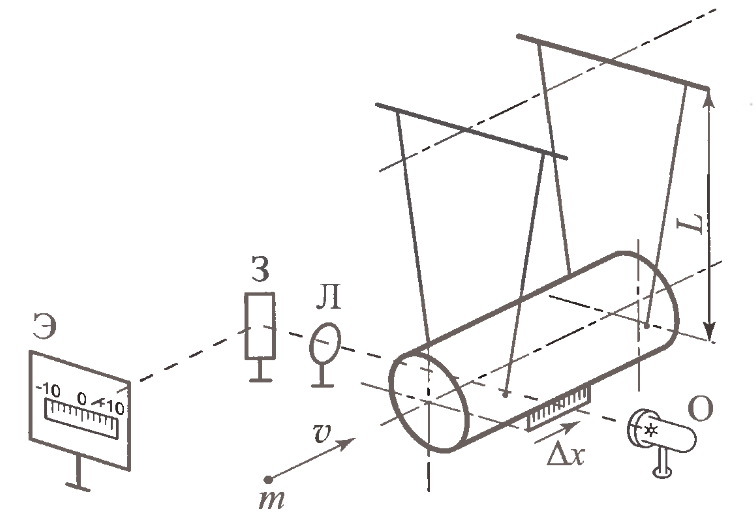
\includegraphics[width = 12cm]{scheme1}}
	\caption{Схема установки для измерения скорости полета пули}
\end{figure} 

При проведении эксперимента необходимо позаботиться о том, чтобы после удара пули колебания маятника происходили в одной плоскости и отсутствовали поперечные движения. Достигается это соответствующей установкой ружья. При этом надо иметь в виду, что вслед за пулей из ружья выходит воздушная струя, которая может оказать влияние на движение маятника и исказить результаты опыта. Поэтому ружье должно располагаться на расстоянии, достаточном для растекания струи. Влияние струи газов на маятник можно оценить с помощью холостого выстрела.

\vspace{0.5cm}
\textbf{I. Метод баллистического маятника, совершающего поступательное движение.}

Используемый в этой части работы баллистический маятник представляет собой тяжелый цилиндр, подвешенный на четырех нитях одинаковой длины. Он изображен на рис. 1 вместе с измерительной системой. Любая точка цилиндра при колебаниях маятника движется по дуге окружности, радиус которой равен расстоянию по вертикали между уровнями верхнего и нижнего концов нитей педвеса. Это поясняется на рис. 2 (вид сбоку, в плоскости колебаний). Все точки цилиндра движутся по дугам окружностей одинакового радиуса относительно соответствующих каждой точке центров, в частности, центр масс $M_0$ переходит в $M_1$ по дуге окружности с центром в точке $O$. Все радиусы одинаковы и обозначены $L$.

\begin{figure}[h!]
	\center{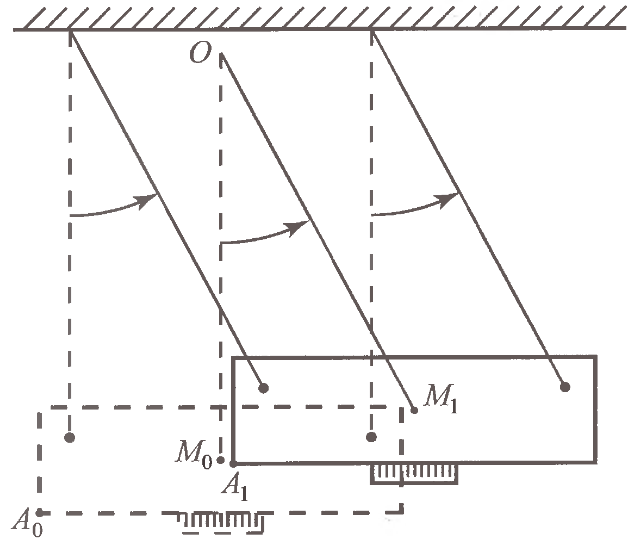
\includegraphics[width = 12cm]{scheme2}}
	\caption{Схема установки для измерения скорости полета пули}
\end{figure} 

Выше уже говорилось о требованиях к установке ружья. В данном случае его необходимо установить таким образом, чтобы скорость пули перед ударом была направлена горизонтально вдоль оси цилиндра (по крайней мере, достаточно близко к этому). Внешними силами для системы пуля-цилиндр являются сила тяжести, которая не имеет горизонтальной компоненты, и силы натяжения нитей, у которых появляются горизонтальные компоненты при отклонении маятника. Однако если отклонения малы, то и эти компоненты малы. Тем более мал по сравнению с импульсом пули их импульс за время соударения. Поэтому закон сохранения импульса при соударении пули с цилиндром имеет вид

\begin{equation}
mu = (M + m)V
\end{equation}

\noindent Здесь $m$ - масса пули, $М$ - масса цилиндра, $u$ - скорость пули перед ударом, $V$ - скорость цилиндра и пули после неупругого соударения. Учитывая, что масса маятника значительно больше массы пули, можно написать 

\begin{equation}
u = \frac{M}{m}V
\end{equation}

Получив начальную кинетическую энергию, маятник при отклонении будет подниматься до тех пор, пока всю ее не израсходует. Если пренебречь потерями, то вся кинетическая энергия переходит в потенциальную в поле тяжести. Тогда по закону сохранения механической энергии высота $h$ подъема маятника над его начальным положением связана с начальной скоростью маятника $V$ следующим образом:

\begin{equation}
V^2 = 2gh
\end{equation}

\noindent Здесь g - ускорение свободною падения.


Высота подъема маятника выражается через угол $\varphi$ отклонения маятника от вертикали:

\begin{equation}
h = L(1 - \cos\varphi) = 2L\sin^2\frac{\varphi}{2},~~~~\text{где}~~~~\varphi \approx \frac{\Delta x}{L}
\end{equation}

Из (2), (3) и (4) получаем окончательную формулу для определения скорости пули:

\begin{equation}
u = \frac{M}{m}\sqrt{\frac{g}{l}}\Delta x
\end{equation}

Измерение отклонения маятника $\Delta x$ производится с помощью оптической системы, изображенной на рис. 1. По увеличенному изображению шкалы, закрепленной на цилиндре, определяется ее горизонтальное смещение. Таким образом может быть измерено максимальное отклонение маятника и изменение максимальных отклонений для определени затуханий колебаний.

Справедливость соотношения (3) и, следовательно, окончательной формулы (5), обусловлена возможностью пренебречь потерями энергии при колебаниях.

Среди причин, вызывающих затухание колебаний маятника, наиболее существенными являются трение о воздух и недостаточно жесткое закрепление точки подвеса.

Если потери энергии за четверть периода колебаний малы по сравнению с максимальной потенциальной энергией, которую маятник при этом приобретает, то их можно не учитывать в законе сохранения (3). Как уже говорилось, затуханием можно пренебречь, если за десять периодов амплитуда колебаний уменьшается меньше, чем в два раза.

\vspace{1cm}
\textbf{Наши действия.}
\vspace{1cm}

\begin{flushleft}
\begin{enumerate}
\item  Измерим на аналитических весах массу каждой пульки, поместим их в ячейки коробки пол соответствующими номерами, чтобы не перепутать при использовании.

\item Измерим с помощью двухметровой линейки расстояние $L$ (рис. 1).

\item Соберем оптическую систему, предназначенную для измерения перемещения маятника. Включим осветитель и добьемся четкого изображения шкалы на экране.

\item Произведем несколько холостых выстрелов по маятнику и убедимся в том, что он практически не реагирует на удар воздушной струи из
ружья.

\item Убедимся в малом затухании колебаний: за десять колебаний амплитуда уменьшается меньше, чем наполовину.

Произведем несколько выстрелов и определим по формуле (5) скорость пули при каждом выстреле.

\item Оценим погрешность определения скорости пули в каждом выстреле.

\item Найдем среднее значение скорости пули и разброс отдельных результатов около среднего значения.
\end{enumerate}
\end{flushleft}

\vspace{1cm}
\textbf{II. Метод крутильного баллистического маятника.}

Схема эксперимента изображена на рис. 3. Пуля массой $m$ попадает в мишень, укрепленную на стержне $aa$, который вместе с грузами $M$ и проволокой $\text{П}$ образует крутильный маятник. Считая удар пули о мишень неупругим, для определения скорости и полета, пули непосредственно перед ударом воспользуемся законом сохранения момента импульса в виде

\begin{equation}
mur = I\Omega
\end{equation}

\noindent Здесь $r$ - расстояние от линии полета пули до оси вращения маятника (до проволоки $\text{П}$), 1 - момент инерции маятника, $\Omega$ - его угловая скорость непосредственно после удара.

\begin{figure}[h!]
	\center{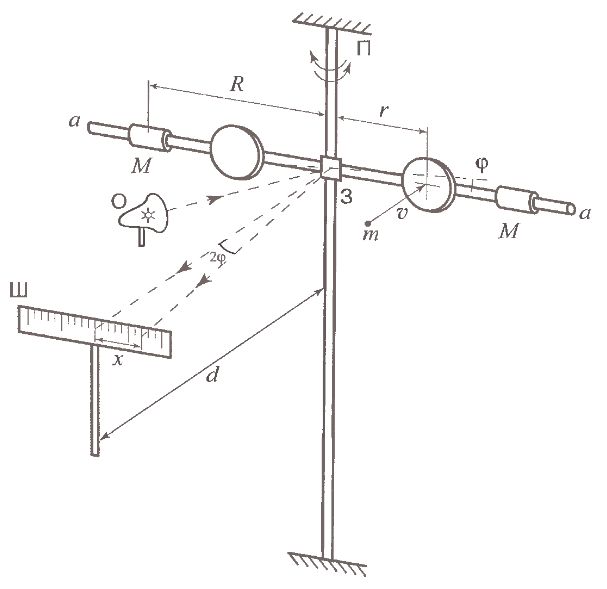
\includegraphics[width = 12cm]{scheme3}}
	\caption{Схема установки для измерения скорости полета пули с крутильным баллистическим маятником}
\end{figure} 

Законом сохранения момента импульса можно воспользоваться, если время соударения пули с мишенью значительно меньше периода малых колебаний маятника. Поворот маятника за время соударения мал по сравнению с максимальным поворотом матяника при колебаниях. Соответственно мал момент кручения, возникающий при этом в проволоке, по сравнению с моментом при максимальном повороте, который всегда имеет конечную величину. Но главное, мало произведение момента кручения в проволоке на время соударения по сравнению с моментом импульса, которым обладала пуля перед ударом.

Начальная кинетическая энергия вращения маятника переходит в потенциальную упругую энергию закручивания проволоки и расходуется на необратимые потери - в первую очередь на трение о воздух. Роль потерь можно оценить по изменению амплитуды колебаний за $10$ периодов. Если амплитуда уменьшается менее чем наполовину, то затухание колебаний считаем малым, то есть потери энергии за период колебаний значительно меньше энергии колебаний. Пренебрегая потерями, закон сохранения энергии при колебаниях записываем следующим образом:

\begin{equation}
k\frac{\varphi^2}{2} = I\frac{\Omega^2}{2}
\end{equation}

\noindent Здесь $k$ - модуль кручения проволоки $\text{П}$, а $\varphi$ - максимальный угол поворота маятника. 

Из (6) и (7) получаем

\begin{equation}
u = \varphi\frac{\sqrt{kI}}{mr}
\end{equation}

Угол максимального закручивания маятника в данных опытах всегда мал и легко находится по смещению $x$ изображения нити осветителя на измерительной шкале. Из рис. 3 следует

\begin{equation}
\varphi \approx \frac{x}{2d}
\end{equation}

\noindent Здесь $d$ - расстояние от шкалы $\text{Ш}$ до оси вращения маятника.

В формулу (8) входит произведение $kI$, которое можно найти по измерениям периодов колебаний маятника c грузами $M$ и без них. В первом случае период колебаний равен

\begin{equation}
T_1 = 2\pi\sqrt{\frac{I}{k}}
\end{equation}

\noindent Во втором случае 

\begin{equation}
T_2 = 2\pi\sqrt{\frac{I - 2MR^2}{k}}
\end{equation}

\noindent Из (10) и (11) следует

\begin{equation}
\sqrt{kI} = \frac{4\pi MR^2T_1}{T_1^2 - T_2^2}
\end{equation}

\noindent Здесь $R$ расстояние от центров масс грузов $M$ до проволоки.

\vspace{1cm}
\textbf{Наши действия.}
\vspace{1cm}

\begin{flushleft}
\begin{enumerate}
\item  Измерим на аналитических весах массу каждой пульки, поместим их в ячейки коробки под соответствующими номерами, чтобы не перепутать при использовании. 

\item  Измерим с помощью линейки расстояния $r$, $R$ и $d$ (см. рис. 3).

\item Настроим оптическую систему, предназначенную для измерения поворота маятника. Включим осветитель $O$, направим свет на зеркальце 
$\text{З}$ и получим четкое изображение нити осветителя на шкале.

\item Произведем  несколько холостых выстрелов и убедимся, что маятник практически не реагирует на воздушную струю из ружья.

\item Убедимся в малом затухании колебаний: за десять колебаний амплитуда уменьшается меньше, чем наполовину.

Измеряя время $10-15$ полных крутильных колебаний маятника, определим $T_1$ и $T_2$. По формуле (12) найдем величину $\sqrt{kI}$ и оценим ее погрешность.

\item Произведем несколько выстрелов и по формулам (9) и (8) определим скорость пули при каждом выстреле.

\item Оценим погрешносгь определения скорости пули при каждом выстреле.

\item Найдем среднее значение скорости пули и разброс отдельных результатов около среднего значения. С чем связан разброс результатов: с погрешностями измерений или с различием скоростей пули в разных  опытах?
\end{enumerate}
\end{flushleft}







\end{document}